\newpage
\section{Architektura}
Nasza biblioteka składa się z wielu współpracujących ze sobą modułów:
\begin{figure}[!ht]
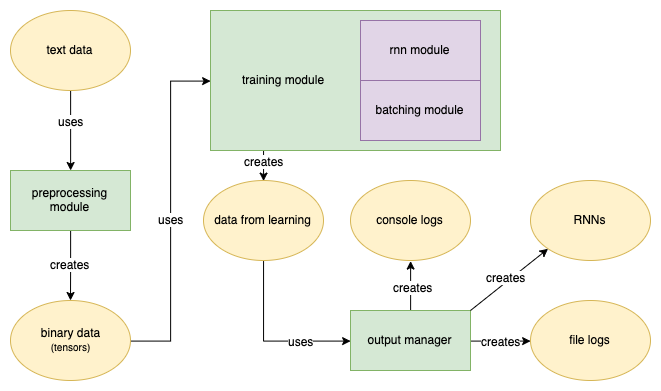
\includegraphics[width=\linewidth]{./images/modules.png}
\caption{schemat modułów biblioteki}
\label{fig:test3}
\end{figure}

\subsection{Moduł preprocesingu}
Największy i całkowicie niezależny od pozostałych części biblioteki moduł, którego zadaniem jest 
przetworzenie tekstów z formy tekstowej na formę binarną (tensory), która jest następnie wykorzystywana
do szkolenia sieci. Na tym etapie następuje również redukcja znaków w tekście, tak by wyeliminować
informacje, które nie są potrzebne z perspektywy szkolenia sieci. Teksty po przetworzeniu są 
zapisywane na dysku i mogą być wykorzystywane wielokrotnie. 
Wadą tego modułu jest długi czas przetwarzania tekstów, która trwa zwykle kilkanaście sekund oraz spora ilość
przestrzeni dyskowej i RAMu które są wykorzystywane w wyniku tego procesu.

\subsection{Moduł batchowania}
Moduł, który korzystając z dostarczonych danych binarnych dzieli je na batche i dostarcza modułowi treningowemu.
Pozwala na specyfikowanie parametrów tych danych, jak na przykład rozmiar batcha.
Decyduje również o tym, kiedy kończy się proces uczenia oraz o losowości ustawienia autorów w batchu. 
Jego kod jest ściśle powiązany z kodem modułu treningu sieci ale z racji na jego obszerność zdecydowaliśmy 
się go wyodrębnić jako osobny moduł. 
Jest on niezależny od modułu preprocesingu, jednak format danych wyjściowych z modułu preprocesingu 
jest zbieżny z formatem danych wejściwych wymaganym przez modułu batchowania. 

\subsection{Moduł sieci} 
Moduł sieci jest małym modułem odpowiedzialnym za deklarację sieci neuronowej w PyTorchu.
 
\subsection{Moduł treningu sieci}
Ten moduł spina moduł sieci oraz moduł batchowania przprowadzając za ich pomocą proces treningu sieci.
To w kodzie tego modułu następuje interacja przez epoki, przekazywanie danych z modułu batchowania 
do sieci, wykorzystanie funkcji kosztu, propagacja wsteczna i wszystkie inne składniki potrzebne do 
szkolenia sieci. 

\subsection{OutputManager}
Ten moduł odpowiedzialny jest za odbieranie danych z modułu treningu sieci, a następnie tworzenie z nich
wygodnego do analizy wyjścia. Wyjście to jest realizowane w formie danych ze szkolenia wyświetlanych 
w konsoli oraz zapisywanych do pliku csv, w formie parametrów sieci, które są zapisywane
w pliku txt oraz w formie kolejnych modeli sieci, które są zapisywane na dysku w formacie\ldots. \TODO{jaki format plikow} 
Logi w konsoli pozowiły nam na wygodne kontrolowanie procesu szkolenia, a dane w plikach csv potrzebne 
nam były do rysowania wykresów.

\newpage
\subsection{Skrypty}
\TODO{zdanie wprowadzające}
\begin{enumerate}
	\item {\texttt{create\_scripts.py} } - 
	tworzy skrypty, które służą do kolejkowania zadań na Prometheusie. Korzysta z pliku konfiguracyjnego \texttt{to\_run.json},
	w którym możemy definiować zarówno parametry sieci, jak i parametry związane ze zlecaniem zadań na Prometheusie.
	Zawartość pliku \texttt{to\_run.json} wraz z przykładowymi parametrami:
	
	\begin{import}
		[
		  {
		    "beginning": "#!/bin/sh",
		    "name": "#SBATCH -J test",
		    "node_numbers": "#SBATCH -N 1",
		    "tasks_per_node": "#SBATCH --ntasks-per-node=1",
		    "mem_per_cpu": "#SBATCH --mem-per-cpu=5GB",
		    "time": "#SBATCH --time=00:20:00",
		    "grant_name": "#SBATCH -A ap2018",
		    "partition": "#SBATCH -p plgrid",
		    "output": "#SBATCH --output=",
		    "errors": "#SBATCH --error=",
		    "hidden_size": "100",
		    "num_layers": "2",
		    "num_epochs": "5",
		    "batch_size": "40",
		    "timesteps": "50",
		    "learning_rate": "0.004",
		    "authors_size": "100",
		    "vocab_size": "48",
		    "save_path": "../results/",
		    "learning_tensors_path": "../data/dutch/tensors/known/",
		    "testing_tensors_path": "../data/dutch/tensors/known/",
		    "language": "DU"
		  }
		]
	\end{import}
	
	Parametry dotyczące zlecania zadań:
	\begin{itemize}
	  \item name - nazwa zlecenia
	  \item node\_numbers - liczba alokowanych węzłów
	  \item task\_per\_node - liczba zadań przypadających na węzeł
	  \item mem\_per\_cpu - ilość pamięci przypadającej na jeden rdzeń obliczeniowy
	  \item time - maksymalny czas trwania zlecenia
	  \item grant\_name - nazwa grantu do rozliczenia zużycia zasobów
	  \item partition - specyfikacja partycji
	  \item output - plik ze standardowym wyjściem
	  \item errors - plik ze standardowym wyjściem błędów
	\end{itemize}
	
	Po wykonaniu komendy \texttt{python3 create\_scripts.py} w katalogu \texttt{scripts} zostaną 
	wygenerowane skrypty pozwalające na uczenie sieci z podanymi parametrami oraz foldery 
	wynikowe dla danej nazwy zlecenia w folderze \texttt{results}. Nazwa zlecenia to ostatni wyraz dla składnika name,
	dla przykładu wyżej byłaby to nazwa \texttt{test}:
	
	\begin{import}
	"name": "#SBATCH -J test",
	\end{import}
	
	W folderze każdego zlecenia inicjalizowane są 4 pliki: 
	
	\begin{itemize}
	  \item network\_info.txt - plik z danymi na temat sieci i parametrami uczenia. Przykładowa zawartość pliku: 
	\begin{import}	
	num_layers: 2
	hidden_size: 100
	batch_size: 1
	timesteps: 40
	learning_rate: 0.004
	num_epochs: 1
	vocab_size: 40
	authors_size: 10
	\end{import}
	  \item output-<nazwa\_zlecenia>.out - plik ze standardowym wyjściem z wywołania programu.
	  \item errors-<nazwa\_zlecenia>.out -  plik gdzie zapisywane są logi z błędami.
	  \item results.csv - plik z danymi z uczenia jak skuteczność, wartość funkcji kosztu, czas uczenia, 
	  numer epoki. Wypełniany jest podczas procesu uczenia sieci. Służy do rysowania wykresów. 
	  Przykładowa zawartość pliku:
	  	  \begin{import}	
id,epoch,loss,accuracy,time
1,1,3.5167935148152436,0.012658227848101266,0:27:30.020267
2,2,1.6148932912132955,0.127848101235212313,0:57:28.588744
3,3,0.8160962337213797,0.312658256743278567,1:27:04.476756
4,4,0.7149949056285243,0.382658226754242341,1:58:06.904183
	  \end{import}
	  
	\end{itemize}
	 
	oraz folder \texttt{models} gdzie zapisywane są pliki z zawartością modelu z poszczególnych epok.
	
	\item {\texttt{run.sh} } - 
	Uruchamia skrypty utworzone poprzez \texttt{create\_scripts.py} odpowiednio je kolejkując. Należy
	pamiętać o wcześniejszej inicjalizacji skryptów z parametrami opisanymi powyżej.
	
	\item {\texttt{copy\_data\_to\_prometheus.sh} } - używany przez nas do przesyłania tekstów po preprocesingu
	bezpośrednio na Prometheusie. 
	
	\item {\texttt{copy\_results\_LOCAL.sh} } - skrypt służący do kopiowania rezultatów uczenia z Prometheusa na 
	na komputer osobisty. Wykonujemy go lokalnie z naszego komputera. 

	\item {\texttt{draw\_plots.py} } - Analizuje dane otrzymane z procesu uczenia i przedstawia je w formie wykresów.
	Uruchumiony szuka folderu \texttt{results }w folderze w którym się aktualnie znajduje. Następnie iteruje po folderach
	wykonanych zadań z folderu \texttt{results}, z każdego z nich czyta plik \texttt{results.csv} i rysuje dla niego wykres epoki od kosztu
 	oraz epoki od skuteczności. Wykresy zapisuje w folderze \texttt{plots}, gdzie plik każdego wykresu ma nazwę 
 	zlecenia, którego dane przedstawia.
 	
 	\begin{figure}[H]
	\centering
	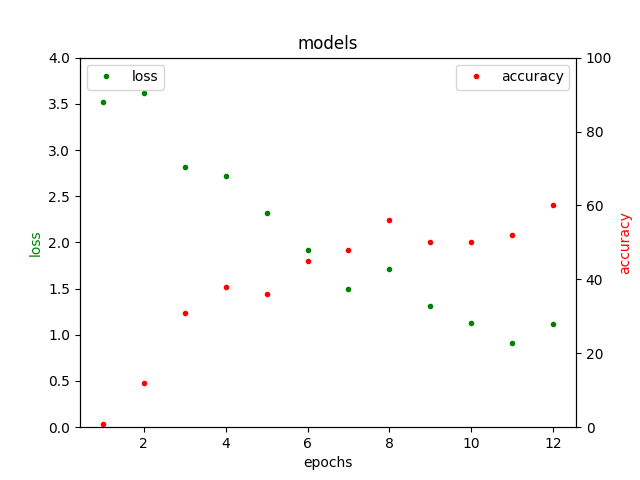
\includegraphics[height=7cm]{./images/plot.png}
	\caption{Przykładowy wykres kosztu od skuteczności}
	\label{fig:test5}
	\end{figure}
 	
	
	\item {\texttt{clean.sh} } - usuwa dotychczasowe wyniki, pliki tymczasowe itp.
	
	\item {\texttt{uncode\_tensor.py} } - skrypt służący do odkowawania tekstu w postaci tablicy wektorów one hot powtórnie do 
 	formy tekstowej. Służył do debugowania sieci, w szczególności sprawdzania czy dane wejściowe oraz 
 	oczekiwane znaki wyjściowe są poprawne.
 	
 	\item {\texttt{list\_lengths.py} } - skrypt służący do listowania łącznej długości tekstów dla każdego z autorów
 	w podanym folderze. Służył do analizy zbioru danych wejściowych.
	
	
	
\end{enumerate}



